% Radiacode Track Analyzer -- short software paper for arXiv.
%
% Build:  make          (needs a TeX distribution; see README.md in this folder)
% Target: arXiv preprint, physics.ins-det (cross-list physics.data-an).
\documentclass[10pt,twocolumn]{article}

% Latin Modern rather than the default Computer Modern. Under T1 encoding the
% CM fonts are METAFONT bitmaps unless cm-super is installed, and microtype's
% font expansion needs scalable outlines -- on a BasicTeX install that is a
% fatal "auto expansion is only possible with scalable fonts". Latin Modern is
% the Type 1 successor to CM, ships with BasicTeX, and looks the same.
\usepackage{lmodern}
\usepackage[T1]{fontenc}
\usepackage[utf8]{inputenc}
\usepackage[margin=1.9cm]{geometry}
\usepackage{amsmath}
\usepackage{graphicx}
\usepackage[hidelinks]{hyperref}
\usepackage{microtype}

\graphicspath{{../docs/}}

\setlength{\parskip}{0pt}
\pagestyle{plain}

% Two pages is the target, and floats plus the bibliography are where the
% slack is. Tightening separation rather than cutting content.
\setlength{\textfloatsep}{8pt plus 2pt minus 2pt}
\setlength{\intextsep}{8pt plus 2pt minus 2pt}
\setlength{\dblfloatsep}{8pt plus 2pt minus 2pt}
\setlength{\abovecaptionskip}{4pt}
\setlength{\belowcaptionskip}{0pt}

\title{\vspace{-1.4em}\large\bf Radiacode Track Analyzer: open-source analysis
of GPS-tagged radiation tracks from consumer CsI(Tl) dosimeters}

\author{\normalsize Lorenzo Confalonieri\\[1pt]
\small The University of Texas at Austin\, ---\,
\texttt{lorenzo.confalonieri@utexas.edu}}

\date{}

\begin{document}
\maketitle

\begin{abstract}
\noindent
\small
The RadiaCode 100-series is a palm-sized CsI(Tl) scintillation dosimeter whose
companion application logs GPS-tagged tracks of count rate and dose rate. The
application maps those tracks but does not analyse them, and the file format is
undocumented. \emph{Radiacode Track Analyzer} (\texttt{rcta}) is an
MIT-licensed Python package --- a headless command-line tool plus an optional
Qt desktop application --- that turns such a track into a quantitative result
with its uncertainty attached. It reports a Currie minimum detectable dose rate
whenever it finds no detection, corrects a multi-scale scan for its
${\sim}2\times10^{4}$ implicit tests, de-weights correlations on a series whose
lag-1 autocorrelation is 0.9985, separates GPS jitter from travelled distance,
and validates imported aircraft altitude against the detector's own fixes
before use. We also give a reverse-engineered specification of the format.
\end{abstract}

\section{Introduction}

Inexpensive scintillation detectors have put mobile radiation measurement
within reach of undergraduate laboratories, environmental surveys and
citizen-science groups. The RadiaCode 100-series is representative: a
palm-sized CsI(Tl) instrument logging count rate and dose rate tagged with GPS
position and horizontal accuracy, so a walk, a drive or a flight each produce
a single file. What the vendor application does with that file is draw it. A
heat-mapped track is persuasive, and a coloured line reads as signal whether or
not one is present; the step to a defensible statement is left to the user, and
the format is undocumented. \texttt{rcta} addresses both gaps, on the premise
that the useful output of a mobile survey is usually a bound, not a
detection.

\section{Implementation}

\texttt{rcta} is pure Python ($\geq$\,3.10) requiring only NumPy and SciPy;
PySide6 and pyqtgraph are an optional extra, so the analysis core runs headless
or in a notebook. The package separates \texttt{core/} (pure NumPy/SciPy, never
imports Qt, never touches the network) from \texttt{net/} and \texttt{gui/},
and those boundaries are enforced by a test module that inspects the import
graph. The suite is 906 tests against ${\sim}13{,}800$ lines, and every
quantitative claim below is pinned by a regression test.

\noindent\begin{minipage}{\columnwidth}\small
\begin{verbatim}
rcta-cli info    TRACK.rctrk
rcta-cli analyze TRACK.rctrk --json report.json
rcta-cli flight  TRACK.rctrk --flight DL2618 \
                 --date 2026-09-07
rcta                       # desktop application
\end{verbatim}
\end{minipage}

Two real acquisitions ship with the package --- a 2\,h walking survey
(Fig.~\ref{fig:walk}) and a 2\,h\,42\,m flight --- so worked examples include
the awkward parts: dropouts, out-of-order samples, 300\,m fixes. The vendor
publishes no specification: the application writes two dialects under one
extension, randomises key order within a record, emits samples out of time
order, and records dose rate in microroentgen per hour without recording the
unit. \texttt{docs/FORMAT.md} is a specification measured against real files
and enforced by tests; the unit was settled against a walking log and the
application's own display, after an earlier parser read the values as nSv/h and
was wrong tenfold.

\begin{figure}[t]
\centering
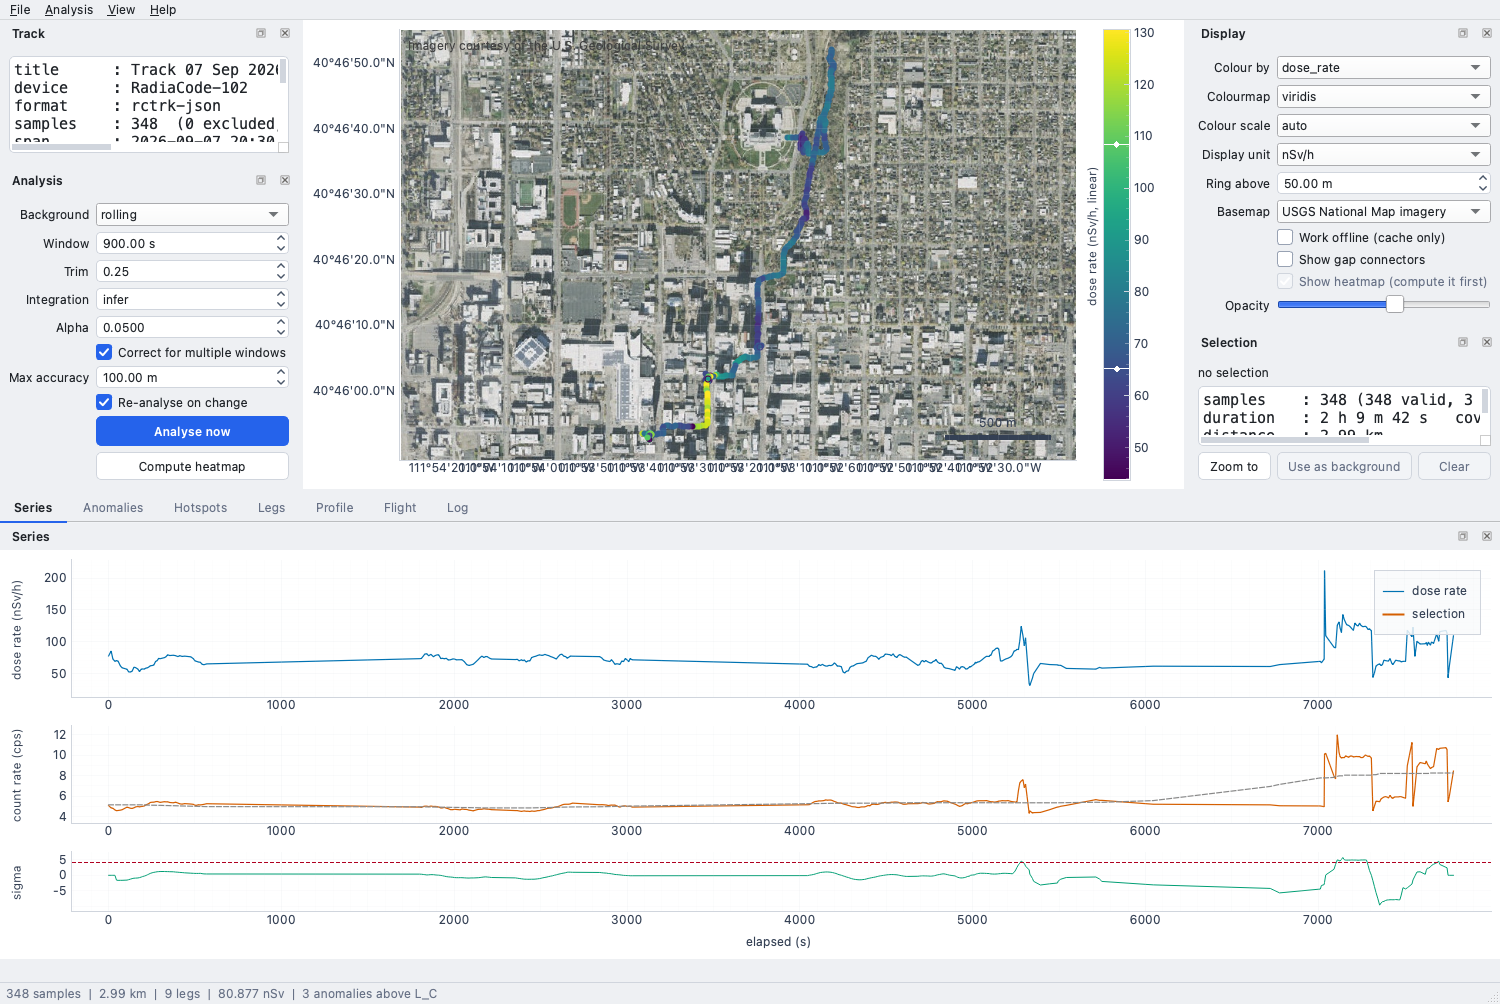
\includegraphics[width=\columnwidth]{screenshot-walk.png}
\caption{A 2\,h walking survey: 348 samples, 2.99\,km, background 5.31\,cps
(70.1\,nSv/h). One feature reaches $7.4\,\sigma$ on two independent passes; a
second, seen once, is only \emph{possible} at $4.6\,\sigma$.}
\label{fig:walk}
\end{figure}

\section{Statistical treatment}

\paragraph{Detection limits.} When nothing exceeds the critical level
$L_\text{C}$, \texttt{rcta} reports the minimum detectable dose rate against
integration window in place of a null verdict --- on the bundled flight,
1160\,nSv/h in a single 2\,s sample against 133\,nSv/h over 128\,s. This makes
the Currie framework~\cite{currie1968} concrete for a moving detector and
exposes the $\sqrt{t}$ trade-off between sensitivity and spatial resolution.
The same data show the energy-dependent dose response~\cite{knoll2010}:
13\,nSv/h per cps on the ground against 51 at cruise, so the ratio is computed
per track rather than assumed.

\paragraph{Multiplicity.} Seven window widths across 2{,}964 samples are
20{,}748 implicit tests. At $\alpha=0.05$ the uncorrected $1.64\,\sigma$
threshold returns of order a thousand ``detections'' from clean data;
Bonferroni moves it to $4.57\,\sigma$ and the count to zero, verified over
forty synthetic background tracks.

\paragraph{Serial dependence.} The count rate has a lag-1 autocorrelation of
0.9985, so correlations carry a Bartlett effective sample
size~\cite{bartlett1946}. For speed against dose rate on the walk, $n=347$
becomes $n_\text{eff}=126$ and $p=0.113$ becomes $p=0.343$; on the flight the
naive and corrected $p$-values differ by more than 270 orders of magnitude. The tool also
states what no $p$-value can: on foot, slowing near something of interest
couples speed to dwell time, so a surviving correlation is confounded.

\paragraph{Estimator and geometry.} Background is a symmetrically trimmed mean
of a rolling window, not a low quantile: the 0.25 quantile of an 18\,cps
Poisson background sits 2.0\,cps below the true mean, which over a 64-sample
window is $5.3\,\sigma$ of detection manufactured by the estimator. Geometry
misleads similarly. At 1.4\,m/s with 2\,s logging each step is 2.8\,m against
an 8\,m fix, so raw summed GPS distance overstates a walk by $5.2\times$
against known truth; smoothing within an automatically selected window lands
within 3\,\% across 3--20\,m accuracy. Interpolated surfaces use
Nadaraya--Watson~\cite{nadaraya1964} with two masks, since a one-dimensional
path cannot support a filled map. Accumulated dose is reported twice ---
80.9\,nSv over the 3{,}856\,s logged against 153.8\,nSv integrating across
dropouts, 47\,\% apart --- and the program declines to choose.

\section{Altitude on airborne tracks}

\begin{figure}[t]
\centering
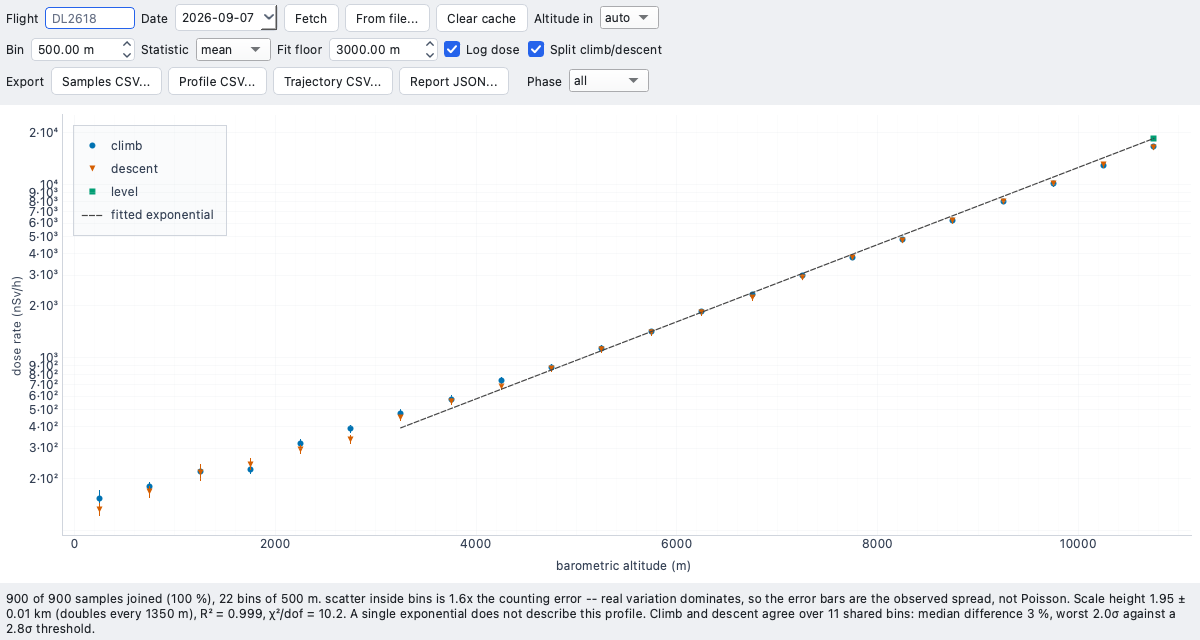
\includegraphics[width=0.94\columnwidth]{screenshot-flight-fit.png}
\caption{Cosmic dose rate against altitude, log ordinate, climb and descent
separate. A constant scale height is a straight line; bins below 3\,km bend
away because terrestrial gamma is altitude-independent, hence the fit floor.}
\label{fig:flight}
\end{figure}

The format carries no altitude, which on an airborne track removes the only
variable that explains the count rate. \texttt{rcta} imports a trajectory ---
from the OpenSky Network~\cite{schafer2014}, or a local file offline --- and
fits an exponential atmosphere (Fig.~\ref{fig:flight}).

The join is the delicate part. \emph{Any} trajectory joins onto \emph{any}
track by timestamp, so a wrong flight, day or leg yields a smooth, plausible,
entirely fictional curve with no symptom: a fabricated altitude axis is
monotonic and the dose really does rise along it. The trajectory's positions
are therefore checked against the recorded fixes, and disagreement beyond
tolerance is a refusal with its own exit code rather than a plot. Because a
clock offset at 233\,m/s is indistinguishable from the wrong flight, the offset
minimising the residual is reported but never applied automatically. Climb and
descent are never pooled: the aircraft crosses the same altitudes twice, hours
apart and a continent away, and their disagreement is the honest error bar on
the fitted scale height.

\section{Limitations and availability}

\texttt{rcta} performs no source localisation or activity estimation, and
tracks carry no spectra, so nuclide identification is impossible from a track
alone. Altitude is validated against position, but a trajectory right in
position may still be wrong in altitude. The per-sample integration time is
inferred from sample spacing because the file does not record it; every
detection limit scales directly with it, which makes it the largest systematic
in the program, and the tool says so on every run. The jitter correction
assumes independent fix errors, so in an urban canyon it is optimistic.

Source, documentation and sample data:
\url{https://github.com/lorenzoconfalonieri/radiacode-track-analyzer}. The
software is MIT licensed; one bundled airport table carrying IANA timezones
from OurAirports (public domain) and OpenFlights (ODbL) is ODbL 1.0, and
analyses made with \texttt{rcta} are Produced Works under that licence with no
share-alike obligation. Trajectory data are provided by the OpenSky
Network~\cite{schafer2014}; basemap tiles by OpenStreetMap contributors and
OpenTopoMap.

\begin{thebibliography}{9}
\footnotesize
\setlength{\itemsep}{0pt}
\setlength{\parskip}{0pt}
\bibitem{currie1968} L.~A. Currie, ``Limits for qualitative detection and
quantitative determination,'' \emph{Anal. Chem.} \textbf{40}, 586--593 (1968).
\bibitem{knoll2010} G.~F. Knoll, \emph{Radiation Detection and Measurement},
4th ed. (Wiley, 2010).
\bibitem{bartlett1946} M.~S. Bartlett, ``On the theoretical specification of
sampling properties of autocorrelated time series,'' \emph{J. R. Stat. Soc.
Suppl.} \textbf{8}, 27--41 (1946).
\bibitem{nadaraya1964} E.~A. Nadaraya, ``On estimating regression,''
\emph{Theory Probab. Appl.} \textbf{9}, 141--142 (1964).
\bibitem{schafer2014} M.~Sch\"afer, M.~Strohmeier, V.~Lenders, I.~Martinovic
and M.~Wilhelm, ``Bringing up OpenSky: A large-scale ADS-B sensor network for
research,'' in \emph{Proc. ACM/IEEE IPSN} (2014), pp.~83--94.
\end{thebibliography}

\end{document}
